\documentclass[12pt]{article}
\usepackage[margin=1in]{geometry} 
\usepackage{amsmath,amsthm,amssymb,amsfonts}
\usepackage{enumerate}
\usepackage{graphicx}
\usepackage{xspace}


\title{APC 523 HW 1}
\author{Samuel Yee}

\begin{document}
\maketitle

\section*{Problem 1}

We can write any real number in binary in terms of a mantissa an exponent:
\begin{equation*}
x = \left(\sum_{l=1}^\infty b_{-l} 2^{-l} \right)\cdot 2^e,
\end{equation*}
where we have taken the convention that the mantissa $m$ is between 0 and 1. In a computer, we have a finite number of bits in which to store the mantissa - for machine numbers in $\mathbb{R}(p, q)$, the mantissa only has $p$ bits. Furthermore, $b_{-1} = 1$. 

One way of obtaining the machine number from the real number is to round the mantissa, such that we round down when the first discarded bit $b_{-(p+1)}=0$, and round up if $b_{-(p+1)} = 1$. 

Consider the first case. Since we are rounding down, the remaining bits $b_{-1}, ... b_{-p}$ are left unchanged. Then
\begin{equation*}
\begin{aligned}
x - \mathrm{rd}(x) &= \left(\sum_{l=1}^\infty b_{-l} 2^{-l} - \sum_{l=1}^p b_{-l} 2^{-l} \right)\cdot 2^e \\
&= \left(\sum_{l=p+1}^\infty b_{-l} 2^{-l} \right)\cdot 2^e \\
&= \left(\sum_{l=p+2}^\infty b_{-l} 2^{-l} \right)\cdot 2^e \\
&\leq 2^{-(p+1)}\cdot 2^e
\end{aligned}
\end{equation*}
The equality in the second to last line is possible because we are in the case $b_{p+1} = 0$. The upper bound on the relative error is thus
\begin{equation*}
\begin{aligned}
\max \left|\frac{x - \mathrm{rd}(x)}{x}\right| &= \frac{2^{-(p+1)}2^e}{2^{-1}\cdot2^e} \\
&= 2^{-p}.
\end{aligned}
\end{equation*}

Now consider the case where we round up, $b_{-(p+1)} = 1$. Then
\begin{equation*}
\begin{aligned}
\mathrm{rd}(x) - x &= \left(\sum_{l=1}^p b_{-l} 2^{-l} + 2^{-p} - \sum_{l=1}^\infty b_{-l} 2^{-l}\right)\cdot 2^e \\
&= \left( 2^{-p} - \sum_{l=p+1}^\infty b_{-l} 2^{-l}\right)\cdot 2^e \\
&\leq \left(2^{-p} - 2^{-(p+1)}\right)\cdot 2^e \\
&= 2^{-(p+1)}\cdot 2^e,
\end{aligned}
\end{equation*}
where the inequality in the second to last line is because $b_{-(l+1)} = 1$, so $\sum_{l=p+1}^\infty b_{-l}2^{-l} \geq 2^{-(p+1)}$. This gives the same relative error as in the first case,
\begin{equation*}
\begin{aligned}
\max \left|\frac{x - \mathrm{rd}(x)}{x}\right| &= \frac{2^{-(p+1)}2^e}{2^{-1}\cdot2^e} \\
&= 2^{-p}.
\end{aligned}
\end{equation*}

Hence the upper bound in the relative error for symmetric rounding is indeed smaller than truncation,
\begin{equation*}
\left|\frac{x-\mathrm{rd}(x)}{x}\right| \leq 2^{-p}.
\end{equation*}

\section*{Problem 2}

\begin{enumerate}[(a)]
\item
Approximating $e^{5.5}$ by its power series up to $n = 30$, truncating each floating point operation at 5 decimal digits, we find
\begin{equation*}
e^{5.5} \approx 244.71.
\end{equation*}

\item
Evaluating each partial sum, we find that the sum converges to five significant figures for $k = 17$. 

The "true" value of $e^{5.5}$, calculated using \texttt{numpy.exp}, is 244.6919323. This gives a relative error of $7.38\times10^{-5}$.

\item
When we compute the partial sums right to left, they converge to 244.69 at $k = 16$, rounded value of the true answer. Thus the relative error incurred when computing the exponential this way is reduced by almost an order of magnitude, $7.90\times10^{-6}$.

This makes sense since when we add right to left, we are adding the smallest terms together, preserving the information in the least significant bits before they are rounded. If we add left to right, small terms are added to a relatively large partial sum and only their most significant bits contribute at all to the sum.

\item
	\begin{enumerate}[(i)]
	\item
	Now, we compute $e^{-5.5} = 0.00408677144$.

	When adding left to right, our procedure converges to $S_k = 0.0038363$, for $k = 25$. This is a relative error of 6.1\%!

	\item
	When we add right to left in each partial sum, the procedure converges to $S_k = 0.0040000$ at $k = 19$. This is both a faster rate of convergence as well as an improved estimate, with a relative error of only 0.021.

	Just as with the postive exponential, adding right to left preserves the least significant bits in the smallest terms. However, both methods give large errors compared with the positive exponential case because they adding terms with alternating signs.

	\item
	Now, we add all the positive (even) terms in the series left to right, but separately from the negative (odd) terms, and finally combine the two. This method converges to a terribly wrong answer of $0.0000$, in $k = 17$ terms.

	Of course, this is to be expected since the two partial sums are close in magnitude but opposite in sign, resulting in catastrophic cancellation.

	\item
	Repeating the same process but computing each partial sum right to left converges to -0.010000 for $k = 18$, even worse than the previous case as it has the wrong sign as the true answer. 

	This should not be unexpected either since adding right to left still leaves both partial sums close in magnitude.
	\end{enumerate}

\item
A better (at least, more accurate) way to compute $e^{-5.5}$ would be to compute $e^{5.5}$ and take the reciprocal. In this way, we avoid the errors that arise from subtracting terms which are close in magnitude as the sum converges.

When we add the partial sums for $e^{5.5}$ right to left and take the reciprocal, our result converges to 0.0040868 after $k = 16$. Once again, this is exactly the correct rounded representation of the true answer, giving a relative error of $6.99\times10^{-6}$. 

\end{enumerate}

\section*{Problem 3}
\begin{enumerate}[(a)]
\item
	\begin{enumerate}[(i)]
	\item
	First, we consider exponentiation of $x$ by a whole-number $n$. One way of computing this is repeated multiplication. Recall that the error in multiplication is
	\begin{equation*}
	\varepsilon(x\cdot y) = \varepsilon_x + \varepsilon_y.
	\end{equation*}

	Thus, repeated multiplication gives the relative error
	\begin{equation*}
	\varepsilon(x^n) = n\varepsilon_x \leq n\cdot\mathrm{eps}.
	\end{equation*}
	
	\item
	We could also compute $x^n = e^{n \ln{x}}$. The error in $n \ln{x}$ is
	\begin{equation*}
	\varepsilon(n\ln{x}) = \varepsilon_{\ln{x}}
	\end{equation*}
	since multiplication by $n$ does not change the relative error. Then

	\begin{equation*}
	\begin{aligned}
	e^{\mathrm{fl}(n\ln{x})} &= e^{(n\ln{x})(1+\varepsilon_{\ln})} \\
	&= e^{n\ln{x}}e^{\varepsilon_{\ln}\left(n\ln{x}\right)} \\
	&\approx e^{n\ln{x}} \left(1 + \varepsilon_{\ln} n\ln{x}\right); \\
	\mathrm{fl}\left[e^{\mathrm{fl}(n\ln{x})}\right] &= \left[e^{n\ln{x}} \left(1 + \varepsilon_{\ln} n\ln{x}\right)\right](1 + \varepsilon_\mathrm{exp}) \\
	&\approx e^{n\ln{x}}\left(1 + \varepsilon_{\exp} + (n\ln{x})\varepsilon_{\ln} \right)
	\end{aligned}
	\end{equation*}

	Thus the error in this computation method is

	\begin{equation*}
	\varepsilon(x^n) = \varepsilon_{\exp} + (n\ln{x})\varepsilon_{\ln} \leq \mathrm{eps}(1 + n\ln{x}).
	\end{equation*}

	This suggests that exponentiation by repeated multiplication is more accurate than the log-exponential method when
	\begin{equation*}
	\begin{aligned}
	n &\leq (1 + n\ln{x}).
	\end{aligned}
	\end{equation*}

	For $x \geq e$, this condition is never satisfied for any whole number $n$.

	For $x < e$, we must have $n \geq 1/(1 - \ln{x})$. This condition is more easily satisfied as $x$ becomes small, and is always satisfied when $x < 1$.

	A general guideline could therefore be to use the log-exponential method for $x \lesssim 1$, and repeated multiplication otherwise, where the exact threshold could be determined empirically.
	\end{enumerate}

\item 
Now suppose we have arbitrary exponents. 

	\begin{enumerate}[(i)]
	\item
	If the exponent $a$ has a relative error $\varepsilon_a$,
	\begin{equation*}
	\begin{aligned}
	x^{\mathrm{fl}(a)} &= x^{a(1+\varepsilon_a)} \\
	&= x^a x^{a \varepsilon_a} \\
	&= x^a e^{a\varepsilon_a\ln{x}} \\
	&\approx x^{a} \left(1 + a\varepsilon_a \ln{x}\right).
	\end{aligned}
	\end{equation*}
	In this case, as assume $x$ is an exact machine number. Hence
	\begin{equation*}
	\varepsilon(x^a) = a \varepsilon_a \ln{x}.
	\end{equation*}
	This error could become large if $a \varepsilon_a$, the absolute error in $a$ is large (e.g. if $a$ is very large). $\ln{x}$ can never be large for any reasonable $x$.


	\item 
	Now if $a$ is an exact machine number but $\mathrm{fl}(x) = x(1 + \varepsilon_x)$, 
	\begin{equation*}
	\begin{aligned}
	\mathrm{fl}(x^a) &= \left[x(1 + \varepsilon_x)\right]^a \\
	&= x^a (1 + \varepsilon_x)^a \\
	&\approx x^a (1 + a \varepsilon_x); \\
	\varepsilon(x^a) &= a\varepsilon_x.
	\end{aligned}
	\end{equation*}

	This can become very large for large $a$. We have seen that in both cases, the relative error is proportional to the size of the exponent.
	\end{enumerate}

\end{enumerate}

\section*{Problem 4}
\begin{enumerate}[(a)]
\item 
We saw in class that the condition number of a scalar function is
\begin{equation*}
\begin{aligned}
\left(\mathrm{cond} f\right)(x) &= \left|\frac{x f'(x)}{f(x)} \right| \\
&= \left|\frac{x e^{-x}}{1-e^{-x}}\right| \\
&= \left|\frac{x}{e^x-1}\right|.
\end{aligned}
\end{equation*}
Since $e^x > x + 1$ for all $x \geq 0$, 
\begin{equation*}
\left(\mathrm{cond} f\right)(x) \leq 1
\end{equation*}
for $x$ on $[0, 1]$.

\item 
Now, suppose that $x$ is a machine number and we perform the given algorithm $A$. Step (i) introduces no error. Evaluating step (ii) yields
\begin{equation*}
\mathrm{fl}(e^{-x}) = e^{-x}(1 + \varepsilon_{\exp}).
\end{equation*}

Step (iii), which is a subtraction, gives
\begin{equation*}
\begin{aligned}
\mathrm{fl}(1 - e^{-x}) &\approx (1 - e^{-x})(1 +e^{-x}\varepsilon_{\exp}).
\end{aligned}
\end{equation*}

Thus in the worst case,
\begin{equation*}
\begin{aligned}
f_A(x) &= f(x) (1 + e^{-x}\mathrm{eps}) \\
&= (1 - e^{-x})(1 + e^{-x + \ln{(\mathrm{eps})}})
\end{aligned}
\end{equation*}

\end{enumerate}


\section*{Problem 5}

We can compute the base $e$ of the natural logarithm using its limit defition, 
\begin{equation*}
e \equiv \lim_{n\rightarrow\infty}\left(1 + \frac{1}{n}\right)^n.
\end{equation*}

Evaluating the argument of the limit for increasing $n = 10^k$, and stopping when we converge over 12 signficant (decimal) figures, we obtain the results in Table \ref{tab:e_approx}.

\begin{table}[h!]
\centering
\begin{tabular}{c|c}
$n$ 		& $\left(1 + 1/n\right)^n$ \\
\hline
$10^{0}$     & 2.00000000000   \\
$10^{1}$     & 2.59374246010   \\
$10^{2}$     & 2.70481382942   \\
$10^{3}$     & 2.71692393224   \\
$10^{4}$     & 2.71814592682   \\
$10^{5}$     & 2.71826823719   \\
$10^{6}$     & 2.71828046910   \\
$10^{7}$     & 2.71828169413   \\
$10^{8}$     & 2.71828179835   \\
$10^{9}$     & 2.71828205201   \\
$10^{10}$    & 2.71828205323   \\
$10^{11}$    & 2.71828205336   \\
$10^{12}$    & 2.71852349604   \\
$10^{13}$    & 2.71611003409   \\
$10^{14}$    & 2.71611003409   \\
\end{tabular}
\caption{Approximation to $e$. \label{tab:e_approx}}
\end{table}

The sequence converges for $n = 10^{13}$, but is in fact only accurate to 3 significant figures. The best approximation to $e = 2.718281828459$ actually occurs for $n = 10^8$, after which the approximation gets worse steadily.

This effect comes from the numerics, since the mathematical limit converges uniformly. What is going on here is that for $n$ powers of ten, $(1 + 1/n)$ does not have finite floating-point representations in binary. Hence when we try to store these values, we lose some information from the mantissa (since the most significant bit is always $1\times2^0$). 

As $n$ gets large, the truncation error relative to $1/n$ gets large, and the machine representation $(1 + 1/n)$ becomes a poorer approximation to the true value. However, since $n$ is stored as an integer, it is exact, and hence we are actually computing the term
\begin{equation*}
\left(1 + \frac{1}{m}\right)^n
\end{equation*}
for some $m \neq n$. 

To fix this, we can either find the correct $m$ and use it for the exponent, or we can simply use powers of two, for which $(1 + 1/n)$ always has a finite representation in floating-point binary.

Indeed, doing the latter converges for $n = 2^{37}$, for which the approximation to $e$ is 2.71828182845, which is indeed accurate down to all but the last significant digit. 


\section*{Problem 6}

In this exercise, we create an array of 1001 floats from 0.0 to 1.0, inclusive. We then successively square-root the array 52 times, followed by squaring it again 52 times. Plotting the result in Figure \ref{fig:sqrt_52}, we see that instead of getting back the original array, we are left with a stepped result, with only 16 unique values.

\begin{figure}[ht!]
\centering
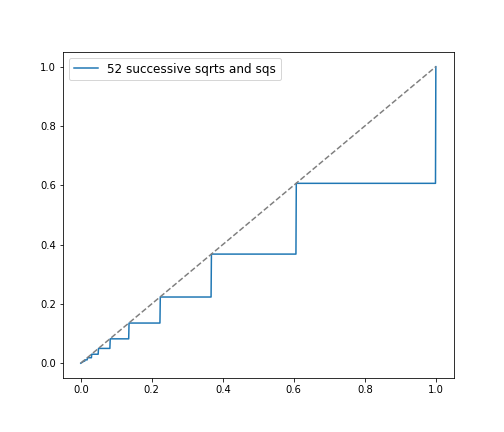
\includegraphics[width=8cm]{sqrt_52.png}
\caption{Taking the square root repeatedly, then squaring repeatedly (52 times).}\label{fig:sqrt_52}
\end{figure}

\begin{figure}[ht!]
\centering
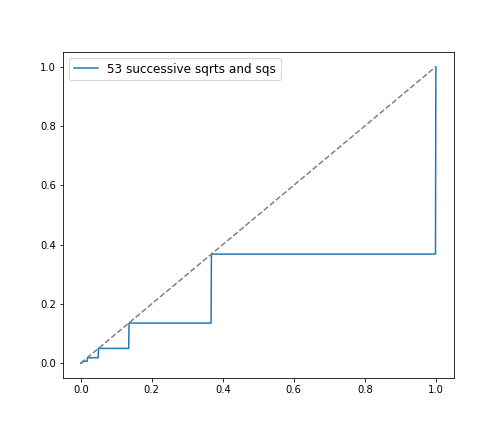
\includegraphics[width=8cm]{sqrt_53.png}
\caption{53 successive square roots and squarings.}\label{fig:sqrt_53}
\end{figure}

To understand what is going on, we examine the second-largest value reached by this process, found to be 0.606530657. Taking the square root of this number 52 times, we get the machine number \texttt{0x1.fffffffffffffp-1} (in hex representation). This is the largest machine number that is still less than one.

Taking the square root of the third-largest value 52 times, we get \texttt{0x1.ffffffffffffep-1}, the next smallest machine number. Indeed, the same process on the remaining unique values in our result array gives us the floating point numbers 0, 1, and \texttt{0x1.fffffffffff2p-1} through \texttt{0x1.ffffffffffffep-1}. 

Why does this happen? When we take the square root of a number between 0.0 and 1.0 repeatedly, the result increases asymptotically to 1.0. However, because of the finite precision of our arithmetic, many starting numbers get mapped to the same numbers close to 1.0.

For example, the smallest non-zero value in our original array, 0.001, gets mapped to 0.9999999999999984 = \texttt{0x1.fffffffffff2p-1}. Since the square root function (and its iterates) are monotonically increasing, all the remaining starting values have to be mapped to the 14 values between \texttt{0x1.fffffffffff2p-1} and \texttt{0x1.ffffffffffffep-1}.

When these values are then squared 52 times, this generates the stepped strucutre we observe in the result. Furthermore, the fixed points are those numbers for which the machine arithmetic exactly maps them onto one of those 14 values.

With this knowledge, we can predict what happens if we have 53 successive square roots. Taking the square root of \texttt{0x1.fffffffffff2p-1} produces \texttt{0x1.fffffffffff9p-1}. This means there are only 7 values that all the numbers in our array are mapped to (apart from 0 and 1), giving a seven-stepped result. This is indeed the case, as can be seen in Figure \ref{fig:sqrt_53}.

\textbf{Note:} I wrote the above before the amendment to the problem was sent out. I've decided not to redo the problem with the new values, but simply provide some additional insight from realizing that if we do the same exercise using numbers between 1.0 and 10.0, we get 1.0, $e$, and $e^2$. 

For numbers greater than 1.0, successive square roots reduces their value asymptotically to 1.0, so in analogy to the above behavior, we expect that many of the numbers will get mapped to values just above 1. In fact, for 52 repetitions, all the numbers in our array get mapped to 1.0, \texttt{0x1.0000000000001p+0} and \texttt{0x1.0000000000002p+0}.

Call $\varepsilon$ = \texttt{0x1.0000000000001p+0} - 1.0 = \texttt{0x1.0000000000000p-52}. Now we see where the magic number of 52 arises from! 

From the limit definition of $e$,
\begin{equation*}
e \equiv \lim_{n\rightarrow\infty}\left(1 + \frac{1}{n}\right)^n.
\end{equation*}

In this case, $1/n = \varepsilon$, $\log_2{n} = 52$. When we square $(1 + \varepsilon)$ repeatedly $k$ times, we are taking it to the power $2^k$. So for $k = 52$, we have
\begin{equation*}
\left(1 + \varepsilon\right)^{1/\varepsilon} \approx e.
\end{equation*}
The second value is $1 + 2\varepsilon$ and becomes
\begin{equation*}
\left(1 + 2\varepsilon\right)^{2/(2\varepsilon)} \approx e^2.
\end{equation*}

In the original problem, taking the values between 0.0 and 1.0, we are doing the same thing except for negative powers, and the values we arrive at are $e^{-1}, e^{-2}, \dots$

If we take the number of loops $k = 53$, then we have
\begin{equation*}
\left(1 + \varepsilon\right)^{2\varepsilon} \approx e^2,
\end{equation*}
so even the value $(1 + \varepsilon)$ gets mapped to $e^2$ and we get only one step.

Conversely, if $k = 51$, then we have more steps, because the initial process of repeated square roots maps the array to between 1.0 and $1.0 + 4\varepsilon$. Furthermore, the locations of the steps is at
\begin{equation*}
\left(1 + n\varepsilon\right)^{\frac{1}{2}(n/n\varepsilon)} \approx e^{n/2}, \quad n=0,1,2,3,4;
\end{equation*}
i.e. we get steps at $e^0, e^{0.5}, e^{1}, e^{1.5}$~and~$e^2$.

Generalizing, for $k$ loops we have
\begin{equation*}
\left(1 + n\varepsilon\right)^{2^{(k-52)}/n\varepsilon} \approx e^{2^{k-52}n}.
\end{equation*}
The number of steps in the final result depends on how many $n$ for which $1.0 \leq e^{2^{k-52}n} < 10.0$. Noting that only $e^0, e^1, e^2$ are within that range, we require
\begin{equation*}
\begin{aligned}
0 &\leq 2^{k-52}n \leq 2 \\
n &\leq 2^{53 - k}.
\end{aligned}
\end{equation*}
i.e. there are a maximum of $2^{53-k}$ steps for $k$ loops. 


\section*{Problem 7}

\begin{enumerate}[(a)]
\item
Here, we are working with Wilkinson's polynomial,
\begin{equation*}
w(x) \equiv \prod_{k=1}^{20}(x-k) = (x-1)(x-2)\cdots(x-20).
\end{equation*}

We can evaluate the coefficients by multiplying out each term recursively using only integer multiplication, where the first term is $(x - 1)$ and the $n$-th term can is
\begin{equation*}
\begin{aligned}
w_{n}(x) &= \left[\prod_{k=1}^{n-1} (x-k)\right](x - n) \\
&= \left[\sum_{k=0}^{n} a_k x^k\right](x - n) \\
&= \sum_{k=0}^{n}a_k x^{k+1} - n\sum_{k=0}^{n}a_k x^{k} \\
&= \sum_{k=1}^{n+1}a_{k-1} x^{k} - n\sum_{k=0}^{n}a_k x^{k}\\
&= a_n x^{n+1} + \sum_{k=1}^n (a_{k-1}-n a_k)x^k -na_0.
\end{aligned}
\end{equation*}

This gives us
\begin{equation*}
\begin{aligned}
w(x) = w_{20}(x) =\,&x^{20} - 210x^{19} + 20615x^{18} - 1256850x^{17} \\
&+ 53327946x^{16} - 1672280820x^{15} \\
&+ 40171771630x^{14} - 756111184500x^{13} \\
&+ 11310276995381x^{12} - 135585182899530x^{11} \\
&+ 1307535010540395x^{10} - 10142299865511450x^{9} \\
&+ 63030812099294896x^{8} - 311333643161390640x^{7} \\
&+ 1206647803780373360x^{6} - 3599979517947607200x^{5} \\
&+ 8037811822645051776x^{4} - 12870931245150988800x^{3} \\
&+ 13803759753640704000x^{2} - 8752948036761600000x \\
&+ 2432902008176640000
\end{aligned}
\end{equation*}

\item 
Creating a polynomial using \texttt{numpy.polynomial.Polynomial}, we can find the roots.

Using \texttt{scipy.optimize.newton}, which is a Newton-Raphson based root-finder, we find the largest root to be at $x = 19.9999949571418$, a relative error of $2.5\times10^{-7}$ from the true value.

Using \texttt{numpy.polynomial.Polynomial.roots()}, the largest root found is $x - 20.0005420937$, giving a relative error of $2.7\times10^{-5}$.


\item 
Now, we perturb the leading coefficient of the polynomial from 1 to $1 + \delta$. We find that the Newton-Raphson method takes longer to converge, and in fact converges to much smaller values as the perturbation increases, as shown in Table \ref{tab:Wilkinson_perturbed}.

\begin{table}[h!]
\centering
\begin{tabular}{c|c|c}
$\delta$ 		& $x_r$ 		& Rel. error \\
\hline
$10^{-8}$	& 9.58539		& 0.521 \\
$10^{-6}$	& 7.75271		& 0.612 \\
$10^{-4}$	& 5.96933		& 0.702 \\
$10^{-2}$	& 5.46959		& 0.727 \\
\end{tabular}
\caption{Largest root found by Newton-Raphson. \label{tab:Wilkinson_perturbed}}
\end{table}


\item 
We can also perturb the second coeffcient, $a_19 = -210$, to a nearby machine number, $-210 - 2^{-23}$. Now, the largest root only changes slightly, to $20.8469$.

If we try to find the next largest root, starting the Newton-Raphson iteration with an initial guess of 19, the method converges to 8.0073.

We can get a clearer picture of what is going on by using the \texttt{numpy.polynomial.Polynomial.roots()} method to get a list of all the roots:
\begin{equation*}
\begin{aligned}
&1.00000,\quad 2.00000,\quad 3.00000,\quad 4.00000,\quad 4.99999, \\
&6.00001,\quad 6.99966,\quad 8.00777,\quad8.91461, \\
&10.09443 - 0.64844i,\quad 10.09443 + 0.64844i, \\
&11.79460 - 1.65426i,\quad 11.79460 + 1.65426i, \\
&13.99301 - 2.51922i,\quad 13.99301 + 2.51922i, \\
&16.73096 - 2.81266i,\quad 16.73096 + 2.81266i, \\
&19.50250 - 1.94033i,\quad 19.50250 + 1.94033i, \\
&20.84693	
\end{aligned}
\end{equation*}

We see that while the nine smallest roots have been only slightly perturbed, ten of the roots have become complex conjugate pairs!


\item 

	\begin{enumerate}[(i)]
	\item

	Consider the monic degree-$n$ polynomial
	\begin{equation*}
	p(x) = \sum_{k=0}^n a_k x^k
	\end{equation*}
	with roots $\Omega_k$, $k = 1,\dots, n$.

	Suppose we perturb the $l$-th coefficient of $p(x)$, such that
	\begin{equation*}
	\widetilde{p}(x) = p(x) + \Delta a_l x^{l}.
	\end{equation*}

	For sufficiently small perturbations, each root $\Omega_k$ of $p(x)$ will have a corresponding root $\widetilde{\Omega}_k$ of $\widetilde{p}(x)$ close to $\Omega_k$. Then the condition number for the $k$-th root given changes to the $l$-th coefficient is

	\begin{equation*}
	\Gamma_{kl} = \left|\frac{\widetilde{\Omega}_k - \Omega_k}{\Omega_k}\right| / \left|\frac{\Delta a_l}{a_l}\right|.
	\end{equation*}

	Taylor expanding $\widetilde{p}(x)$ around $\Omega_k$ assuming $(\widetilde{\Omega}_k - \Omega_k)$ is small, 
	\begin{equation*}
	\begin{aligned}
	\widetilde{p}(\Omega_k) &\approx \widetilde{p}(\widetilde{\Omega}_k) + (\Omega_k - \widetilde{\Omega}_k)\widetilde{p}'(\widetilde{\Omega}_k) \\
	&= (\Omega_k - \widetilde{\Omega}_k)\left(p'(\widetilde{\Omega}_k)+ l\Delta a_l\widetilde{\Omega}_k ^{l-1}\right) \\
	&\approx (\Omega_k - \widetilde{\Omega}_k)p'(\Omega_k).
	\end{aligned}
	\end{equation*}
	In the last line, we have neglected the second order term $\Delta\Omega_k\Delta a_l$ and taken $\Delta\Omega_k p'(\widetilde{\Omega}_k) = \Delta\Omega_k [p'(\Omega_k) + O(\Delta\Omega_k] \approx \Delta \Omega_k p'(\Omega_k)$.

	But also,
	\begin{equation*}
	\begin{aligned}
	\widetilde{p}(\Omega_k) &= p(\Omega_k) + \Delta a_l \Omega_k^l \\
	&= \Delta a_l \Omega_k^l.
	\end{aligned}
	\end{equation*}

	Thus, we have
	\begin{equation*}
	\begin{aligned}
	\left|\frac{\widetilde{\Omega}_k - \Omega_k}{\Omega_k}\right| &= 
	\left|\frac{1}{\Omega_k} \frac{\widetilde{p}(\Omega_k)}{p'(\Omega_k)}\right| \\
	&= \left|\frac{1}{\Omega_k} \frac{\Delta a_l \Omega_k^l}{p'(\Omega_k)}\right|.
	\end{aligned}
	\end{equation*}

	Then the condition number is
	\begin{equation*}
	\Gamma_{kl} = \left|\frac{a_l \Omega_k^{l-1}}{p'(\Omega_k)}\right|.
	\end{equation*}

	For the $k$-th root, we thus have
	\begin{equation*}
	\begin{aligned}
	(\mathrm{cond}\,\Omega_k)(\vec{a}) = \sum_{l=0}^{n-1}\left|\frac{a_l \Omega_k^{l-1}}{p'(\Omega_k)}\right|.
	\end{aligned}
	\end{equation*}

	\item
	We can calculate the condition numbers for the roots of the Wilkinson polynomial. We note that 
	\begin{equation*}
	\begin{aligned}
	w'(x) &= \sum_{l=0}^{n-1} (l+1) a_{l+1} x^l.
	\end{aligned}
	\end{equation*}

	The condition numbers for some of the roots are summarized in Table \ref{tab:wilkinson_condition}. We see that even the slightest perturbation in the coefficients gets amplified massively when finding the roots.


	\begin{table}[h!]
	\centering
	\begin{tabular}{c|c}
	Root & $\mathrm{cond}\,(r)$ \\
	\hline
	14	& $5.40\times10^{13}$ \\
	16  & $3.54\times10^{13}$ \\
	17  & $1.81\times10^{13}$ \\
	20. & $1.38\times10^{11}$ \\
	
	\end{tabular}
	\caption{Condition numbers for Wilkinson's polynomial. \label{tab:wilkinson_condition}}
	\end{table}

	\item 
	Because it is the polynomial whose roots are to be found that is ill-conditioned, even the best algorithm will not be able to help significantly. Because of the large condition numbers, an error as small as the machine epsilon will still result in big discrepancies in the final result.

	\end{enumerate}

\end{enumerate}

\section*{Problem 8}
\begin{enumerate}[(a)]
\item
Reversing the recurrence relation, we get:
\begin{equation*}
y_{n-1} = \frac{e - y_n}{n}.
\end{equation*}

\item
At each iteration, the error in $y_{n-1}$ shrinks, with
\begin{equation*}
\begin{aligned}
\delta y_{n-1} &= \frac{e - (y_n + \delta y_n)}{n} - \frac{e - y_n}{n} \\
&= -\frac{\delta y_n}{n} \\
\left|\frac{\delta y_{n-1}}{y_{n-1}}\right| / \left|\frac{\delta y_{n}}{y_{n}}\right| &= \frac{1}{n}\frac{y_n}{y_{n-1}} \\
&< \frac{1}{n}
\end{aligned}
\end{equation*}
since $y_{n} < y_{n-1}$. If $g_k$ represents the map taking $y_N$ to $y_k$ for some $k < N$, the condition number for $g_k$ is
\begin{equation*}
\begin{aligned}
(\mathrm{cond}\,g_k)(y_N) &< \prod_{n=N}^{k+1}\frac{1}{n} \\
&= \frac{k!}{N!} \\
&< \left(\frac{1}{N}\right)^{N-k-1}.
\end{aligned}
\end{equation*}


\item 
Suppose we start with $y_N^* = 0, \delta y_N / y_N = 1$. The relative error shrinks, such that
\begin{equation*}
\begin{aligned}
\frac{\delta y_k}{y_k} &\leq \frac{\delta y_N}{y_N} \frac{1}{N^{N-k-1}}.
\end{aligned}
\end{equation*}

To achieve a relative error of $\varepsilon$ in $y_k$, we therefore require
\begin{equation*}
\begin{aligned}
\frac{1}{N^{N-k-1}} &< \varepsilon \\
(N - k - 1)\ln{N} &> -\ln{\varepsilon} \\
(N - k - 1)\ln{(N-k-1)} &> -\ln{\varepsilon}
\end{aligned}
\end{equation*}
which we can solve numerically once for a given desired machine epsilon $\varepsilon = \mathrm{eps}$, to determine how far down from $k$ we have to start the iteration.


\item 
The machine epsilon is $\mathrm{eps} = 2.22\times10^{-16}$ for 64-bit floats. Solving the equation above, we find that we require $(N - k - 1) > 13.7$, or $N > k + 15$.

For $k = 20$, we only need to start at $N = 35$. Peforming the calcuation, we achieve a result of $y_{20} = 0.1238038307625699$.

The result from Mathematica is $y_{20} = 0.1238038307625704$, giving an absolute difference of $5\times10^{-16}$ and a relative difference of $4.0\times10^{-15}$. 

Meanwhile, using the built-in \texttt{scipy.integrate.quad} function, we get a result of $y_{20} = 0.12380383076256998$, almost identical. 

Thus, all these methods achieve similar results but certainly the recurrence relation uses the fewest operations, requiring only $\sim 30$ subtractions and divisions.




\end{enumerate}
\end{document}

































